%%%%%%%%%%%%%%%%%%%%%%%%%%%%%%% beamer %%%%%%%%%%%%%%%%%%%%%%%%%%%%%%%%%%%%%%%%%%%%%%%%%
% To run - pdflatex filename.tex
% acroread filename.pdf
%%%%%%%%%%%%%%%%%%%%%%%%%%%%%%%%%%%%%%%%%%%%%%%%%%%%%%%%%%%%%%%%%%%%%%%%%%%%%%%%%%%%%%%% 

\documentclass[compress,red]{beamer}
\mode<presentation>

\usetheme{Warsaw}
% other themes: AnnArbor, Antibes, Bergen, Berkeley, Berlin, Boadilla, boxes, CambridgeUS, Copenhagen, Darmstadt, default, Dresden, Frankfurt, Goettingen,
% Hannover, Ilmenau, JuanLesPins, Luebeck, Madrid, Maloe, Marburg, Montpellier, PaloAlto, Pittsburg, Rochester, Singapore, Szeged, classic

% \usecolortheme{lily}
% color themes: albatross, beaver, beetle, crane, default, dolphin, dov, fly, lily, orchid, rose, seagull, seahorse, sidebartab, structure, whale, wolverine

% \usefonttheme{serif}
% font themes: default, professionalfonts, serif, structurebold, structureitalicserif, structuresmallcapsserif

\hypersetup{pdfpagemode=FullScreen} % makes your presentation go automatically to full screen

% define your own colors:
\definecolor{Red}{rgb}{1,0,0}
\definecolor{Blue}{rgb}{0,0,1}
\definecolor{Green}{rgb}{0,1,0}
\definecolor{magenta}{rgb}{1,0,.6}
\definecolor{lightblue}{rgb}{0,.5,1}
\definecolor{lightpurple}{rgb}{.6,.4,1}
\definecolor{gold}{rgb}{.6,.5,0}
\definecolor{orange}{rgb}{1,0.4,0}
\definecolor{hotpink}{rgb}{1,0,0.5}
\definecolor{newcolor2}{rgb}{.5,.3,.5}
\definecolor{newcolor}{rgb}{0,.3,1}
\definecolor{newcolor3}{rgb}{1,0,.35}
\definecolor{darkgreen1}{rgb}{0, .35, 0}
\definecolor{darkgreen}{rgb}{0, .6, 0}
\definecolor{darkred}{rgb}{.75,0,0}

\xdefinecolor{olive}{cmyk}{0.64,0,0.95,0.4}
\xdefinecolor{purpleish}{cmyk}{0.75,0.75,0,0}

% can also choose different themes for the "inside" and "outside"

% \usepackage{beamerinnertheme_______}
% inner themes include circles, default, inmargin, rectangles, rounded

% \usepackage{beamerouterthemesmoothbars}
% outer themes include default, infolines, miniframes, shadow, sidebar, smoothbars, smoothtree, split, tree

\useoutertheme[subsection=false]{smoothbars}

% to have the same footer on all slides
% \setbeamertemplate{footline}[text line]{STUFF HERE!}
\setbeamertemplate{footline}[text line]{} % makes the footer EMPTY

% include packages
\usepackage{helvet}
\usepackage[utf8]{inputenc}
\usepackage[english,bulgarian]{babel}
\usepackage[T2A]{fontenc}

\usepackage{listings}
\lstset{language=Java,
  captionpos=b,
  tabsize=4,
  keywordstyle=\color{blue},
  commentstyle=\color{gray},
  stringstyle=\color{green},
  numbers=left,
  breaklines=true,
  showstringspaces=false,
  basicstyle=\ttfamily,
  emph={label},
  frame=shadowbox, 
  rulesepcolor=\color{blue},
  columns=fixed}

%%%%%%%%%%%%%%%%%%%%%%%%%%%%%%%%%%%%%%%%%%%%%%%%%%%%%%%%%%%%%%%%%%%%%%%%%%%%%%%%%%%%%%%%%% 
%%%%%%%%%%%%%%%%%%%%%%%%%%%%%% Title Page Info %%%%%%%%%%%%%%%%%%%%%%%%%%%%%%%%%%%%%%%%%%%
%%%%%%%%%%%%%%%%%%%%%%%%%%%%%%%%%%%%%%%%%%%%%%%%%%%%%%%%%%%%%%%%%%%%%%%%%%%%%%%%%%%%%%%%%% 

\title{Модерни програмни езици за JVM}
\subtitle{Groovy, Scala и Clojure}
\author{инж. Божидар Бацов}
\institute{OpenFest 2010}
\date{21.11.2010}

%%%%%%%%%%%%%%%%%%%%%%%%%%%%%%%%%%%%%%%%%%%%%%%%%%%%%%%%%%%%%%%%%%%%%%%%%%%%%%%%%%%%%%%%%% 
%%%%%%%%%%%%%%%%%%%%%%%%%%%%%% Begin Your Document %%%%%%%%%%%%%%%%%%%%%%%%%%%%%%%%%%%%%%%
%%%%%%%%%%%%%%%%%%%%%%%%%%%%%%%%%%%%%%%%%%%%%%%%%%%%%%%%%%%%%%%%%%%%%%%%%%%%%%%%%%%%%%%%%% 

\begin{document}

%%%%%%%%%%%%%%%%%%%%%%%%%%%%%%%%%%%%%%%%%%%%%%%%%%%%%%%%%%%%%%%%%%%%%%%%%%%%%%%%%%%%%%%%%% 

\frame{
  \titlepage 
}

%%%%%%%%%%%%%%%%%%%%%%%%%%%%%%%%%%%%%%%%%%%%%%%%%%%%%%%%%%%%%%%%%%%%%%%%%%%%%%%%%%%%%%%%%% 

% \section[Outline]{}	% this puts the outline before EACH section automatically & will highlight the section you're about to talk about
% \frame{\tableofcontents}

%%%%%%%%%%%%%%%%%%%%%%%%%%%%%%%%%%%%%%%%%%%%%%%%%%%%%%%%%%%%%%%%%%%%%%%%%%%%%%%%%%%%%%%%%% 

\section{Въведение}
\subsection{Общи приказки }
\begin{frame}{Кой е инж. Божидар Бацов?}
  \transdissolve
  \pause
  \begin{itemize}
  \item Батман \pause
  \item Хакер \pause
  \item Технически директор на Drow Ltd. \pause
  \item Ентусиаст на тема свободни технологии, качествен алкохол и
    добра музика \pause
  \item Кинокритик на свободна практика \pause
  \item Преподавател на още по-свободна практика \pause
    \item Контакти
      \begin{itemize}
        \item Twitter - bbatsov
        \item Ел. поща - bozhidar@drow.bg
        \item Jabber/GTalk - bozhidar.batsov@gmail.com
        \item irc.freenode.net - bozhidar \#emacs \#clojure \#scala \#lisp
      \end{itemize}
  \end{itemize}
\end{frame}

\subsection{Езикът и платформата Java}

%%%%%%%%%%%%%%%%%%%%%%%%%%%%%%%%%%%%%%%%%%%%%%%%%%%%%%%%%%%%%%%%%%%%%%%%%%%%%%%%%%%%%%%%%% 

\begin{frame}
  \begin{center}
    \begin{block}{Забележка \#1}
      \vspace{.1cm}
      \begin{center} \large
	Аз \textcolor{darkgreen}{НЕ} съм експерт в областта на
        езиците, за които ще си говорим.\\ \vspace{.1cm}
      \end{center}
    \end{block}
    \vspace{1cm}
    \begin{block}{Забележка \#2}
      \vspace{.1cm}
      Тази презентация ще представи само най-общо и повърхностно разглежданите езици.\\ \vspace{.1cm}
    \end{block}
  \end{center}
\end{frame}

\begin{frame}{Java}
  \transdissolve
  \begin{itemize}
  \item Програмен език \pause
  \item Виртуална машина \pause
  \item Стандартна библиотека
  \end{itemize}
\end{frame}

\begin{frame}{Платформата Java}
  \transdissolve
  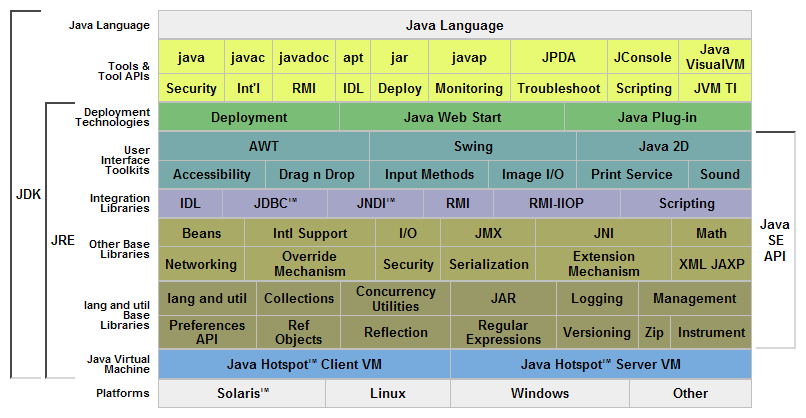
\includegraphics[height=200px, width=320px]{images/JavaPlatform.png}
\end{frame}

\begin{frame}{Езикът Java}
  \transdissolve
    \begin{itemize}
      \item Създаден да замени C++ \pause
      \item Отвежда С++ програмистите до средата на пътя към Lisp \pause
      \item Разработката му е тромава и консервативна \pause
      \item Основни критики към Java в момента
        \begin{itemize}
          \item ниско ниво на изразителност \pause
          \item проповядва императивен стил на програмиране \pause
          \item липсват closures \pause
          \item езикът не е чисто обектно ориентиран \pause
          \item checked exceptions са наказание от Горе \pause
          \item няма възможност за презареждане на оператори \pause
          \item и мнооого други ;-)
        \end{itemize}
    \end{itemize}
\end{frame}

\begin{frame}{Алтернативните езици}
  \transdissolve
  \begin{itemize}
  \item Java 1.0 излиза през януари 1996 \pause
  \item през 1997 вече има 40 езика с имплементации за JVM \pause
  \item през 2004 те са вече 169 \pause
  \item понастоящем са около 240+ \pause
  \end{itemize}
\end{frame}

\begin{frame}{Предимства на разработка на езици за JVM}
  \transdissolve
  \begin{itemize}
  \item Rock solid, hearth touching ;-) \pause
  \item JVM е изключително надеждна, многоплатформена и притежава
    висока производителност и отлични оптимизации \pause
  \item Имате на разположение директно огромната база от съществуващ
    Java код  \pause
  \item Купища отлични инструменти за разработка и привеждане в
    експлоатация
  \end{itemize}
\end{frame}

\begin{frame}{Не всичко е ток и жица}
  \transdissolve
  \begin{itemize}
  \item Виртуалната машина по настоящем не е оптимизирана за динамични
    езици и за някои стилове на програмиране(например функционално) \pause
  \item Виртуалната машина има сравнително голям период на
    студено стартиране(cold start) \pause
  \item Java имплементациите на някои езици като Python(Jython) не са
    съвместими с native имплементациите
  \end{itemize}
\end{frame}

\section{Groovy}
\subsection{Основни характеристики на Groovy}
\subsection{Groovy в действие}

\begin{frame}{Groovy}
  \transdissolve
  \begin{center}
    \begin{block}{Хвала на Groovy} 
    \begin{center}Groovy is like a super version of Java. It can leverage
   Java's enterprise capabilities but also has cool productivity
   features like closures, builders and dynamic typing. If you are a
   developer, tester or script guru, you have to love Groovy.
  \end{center}
  \end{block}
  \end{center}
\end{frame}

\begin{frame}{Пейзажът на JVM езиците}
  \transdissolve
  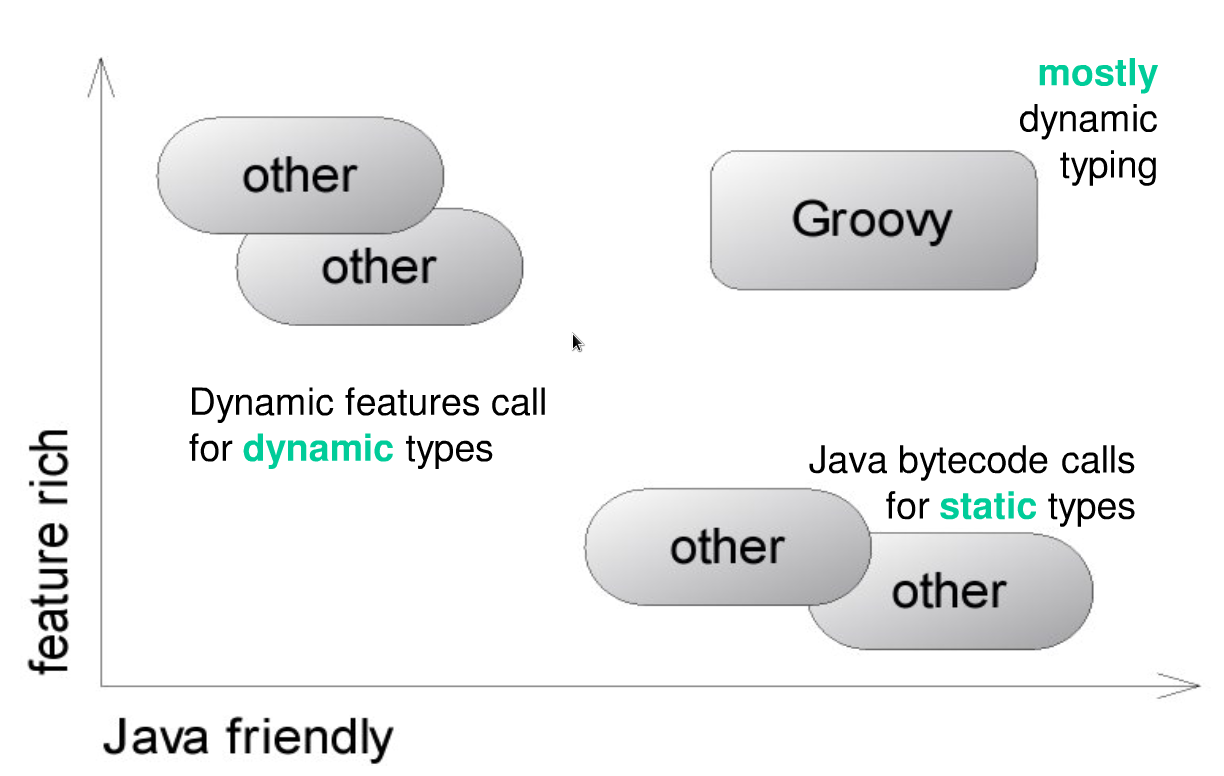
\includegraphics[width=320px, height=150px]{images/landscape.png}
\end{frame}

\begin{frame}{Groovy е...}
  \transdissolve
  \begin{itemize}
  \item Динамичен език за JVM
    \begin{itemize}
      \item Програмите на Groovy директно се компилират до байт код
    \end{itemize}
  \item Вдъхновен от езици като Ruby, Python и Smalltalk
  \item Създаден за да улесни живота на (Java) програмистите
  \item Проект с отворен код, лицензиран под Apache Public License
  \item С граматика директно извлечена от Java 5
    \begin{itemize}
      \item поддържа анотации, generics, изброени типове(enums),
        статични импорти и т.н.
    \end{itemize}
  \end{itemize}
\end{frame}

\begin{frame}{Ключови характеристики}
  \transdissolve
  \begin{itemize}
  \item Напълно обектно-ориентиран
  \item Типизирането не е задължително
  \item Няма нужда да чакате Java 7/8/9:
    \begin{itemize}
      \item Closures - преизползваеми / присвоими блокове код
      \item Атрибути - автоматично генерирани getter/setter методи
    \end{itemize}
  \item Duck typing - типът на обектите се определя от техния
    интерфейс, а не от техния клас
  \item Аритметика базирана на BigDecimal
  \item Улеснена работа с SQL, XML, Swing и т.н.
  \end{itemize}
\end{frame}

\begin{frame}{Java интеграция}
  \transdissolve
  \begin{itemize}
  \item Groovy генерира Java байткод за JVM
    \begin{itemize}
      \item Същите низове, регулярни изрази и т.н.
      \item Същите API
      \item Същия модел на сигурност, същия нишков модел
      \item Същите ОО концепции
      \item Комбинирана компилация
    \end{itemize}
  \end{itemize}
\end{frame}

\subsection{Синтаксис на Groovy}
\begin{frame}[fragile]
  \frametitle{Пример 1}
  \transdissolve
\begin{lstlisting}[basicstyle=\small]
System.out.println("Hello, World!");
println 'Hello, World!'
                       
def name = 'Bozhidar'
println "$name, I'll get the car." // GString
String longer = """${name}, the car
is in the next row."""

def printSize(obj) { 
  print obj?.size() // safe dereferencing
}
 
def pets = ['ant', 'bee', 'cat']

pets.each { pet ->
  assert pet < 'dog'
}
\end{lstlisting}
\end{frame}

\begin{frame}[fragile]
  \frametitle{Пример 2}
  \transdissolve
\begin{lstlisting}[basicstyle=\small ]
import static java.util.Calendar.getInstance as now
import java.util.GregorianCalendar as D
import org.codehaus.groovy.runtime.TimeCategory

println new D(2007,11,25).time
println now().time

assert "Hello World!" =~ /Hello/
// Find operator
assert "Hello World!" ==~ /Hello\b.*/ // Match operator
def p = ~/Hello\b.*/
// Pattern operator
assert p.class.name == 'java.util.regex.Pattern'
\end{lstlisting}
\end{frame}

\begin{frame}{Синтактични конструкции}
  \transdissolve
  \begin{itemize}
  \item Списъци(lists)
    \begin{itemize}
    \item def numbers = [1, 2, 3]      
    \end{itemize}
  \item Асоциативни масиви(maps)
    \begin{itemize}
    \item def map = [BG: "`Bulgaria", DE: "`Germany"]      
    \end{itemize}
  \item Обхват(range)
    \begin{itemize}
      \item def range = 1..1000
    \end{itemize}
  \item Регулярни изрази
    \begin{itemize}
      \item def whitespace = ~/\\s+/
    \end{itemize}
  \end{itemize}
\end{frame}

\subsection{Интересни Groovy API}
\begin{frame}[fragile]
  \frametitle{Groovy Dev Kit(GDK)}
  \transdissolve
  \begin{itemize}
  \item Groovy "`декорира" съществуващите JDK API
  \begin{itemize}
    \item Не можем да разширим java.lang.String или java.io.File?
  \end{itemize}
  \end{itemize}
  \begin{lstlisting}
new File('/x.txt').eachLine {
  println it
}
  \end{lstlisting}

\end{frame}

\begin{frame}{Обработка на данни от външни източници}
  \transdissolve
  \begin{itemize}
    \item Вместо по-добро SQL API имаме стандартен достъп до
      данни(Uniform Data Access)
    \item Достъпът до данни представени като обектни, XML или
      релационни бази данни има повече общи черти, отколкото различни
    \item Едно API независимо от източника на данни
    \item Разликите са само в установяването на изходната постановка
    \item Приликите са в обработката на данните в резултатните структури
    \item Резултатът е подобен на LINQ в .NET
  \end{itemize}
\end{frame}

\begin{frame}[fragile]
  \frametitle{Работа с XML}
  \transdissolve
\begin{lstlisting}[basicstyle=\tiny,language=XML]
<records>
  <car name='HSV Maloo' make='Holden' year='2006'>
    <country>Australia</country>
    <record type='speed'>Production Pickup Truck with speed of 271kph</record>
  </car>
  <car name='P50' make='Peel' year='1962'>
    <country>Isle of Man</country>
    <record type='size'>Smallest Street-Legal Car at 99cm wide and 59 kg weight</record>
  </car>
  <car name='Royale' make='Bugatti' year='1931'>
    <country>France</country>
    <record type='price'>Most Valuable Car at $15 million</record>
  </car>
</records>
\end{lstlisting}
\end{frame}

\begin{frame}[fragile]
  \frametitle{Работа с XML}
  \transdissolve
\begin{lstlisting}
def records = new XmlParser().parse("records.xml")
records.car.each {
  println "year = ${it.@year}"
}
\end{lstlisting}
\end{frame}

\begin{frame}[fragile]
  \frametitle{Swing}
  \transdissolve
\begin{lstlisting}[basicstyle=\tiny]
import java.awt.FlowLayout
builder = new groovy.swing.SwingBuilder()
langs = ["Groovy", "Ruby", "Python", "Pnuts"]
gui = builder.frame(size: [290, 100],
title: 'Swinging with Groovy!') {
panel(layout: new FlowLayout()) {
      panel(layout: new FlowLayout()) {
      for (lang in langs) {
        checkBox(text: lang)
      }
}
button(text: 'Groovy Button', actionPerformed: {
builder.optionPane(message: 'Indubitably Groovy!').
createDialog(null, 'Zen Message').show()
})
button(text: 'Groovy Quit',
actionPerformed: {System.exit(0)})
}
}
gui.show()
\end{lstlisting}
\end{frame}

\begin{frame}{Инструментите на занаята}
  \transdissolve
  \begin{itemize}
    \item Част от дистрибуцията на Groovy
  \begin{itemize}
  \item groovysh
  \item groovyconsole
  \item groovyc
  \end{itemize}
    \item Среди за разботка
      \begin{itemize}
      \item IntelliJ IDEA is the King!
      \item NetBeans
      \item Eclipse
      \end{itemize}
  \item Строителни инструменти
    \begin{itemize}
      \item Apache Maven
      \item Gradle
      \item Apache Buildr
    \end{itemize}
  \end{itemize}
\end{frame}

\section{Scala}
\subsection{Основни характеристики на Scala}
\subsection{Scala в действие}

\begin{frame}{Scala}
  \transdissolve
  \begin{center}
    \begin{block}{James Gosling, създател на Java}
      \begin{center}
        If I were to pick a language
        to use today other than Java,
        it would be Scala...
      \end{center}
    \end{block}    
  \end{center}
\end{frame}

\begin{frame}{Scala e ...}
  \transdissolve
  \begin{itemize}
  \item SCAlable LAnguage
  \item Чист ОО език
  \item Функционален език
  \item Език със статично типизиране
  \item Голяма общност
  \item Прекрасна интеграция със съществуващ Java код
  \end{itemize}
\end{frame}

\begin{frame}[fragile]
  \frametitle{Експресивен}
  \transdissolve
\begin{lstlisting}
val phonebook = Map("Pesho" -> 123456,
                    "Vankata" -> 654321)
phonebook += ("Marmota" -> 987654)
println(phonebook("Pesho"))
\end{lstlisting}
\end{frame}

\begin{frame}[fragile]
  \frametitle{Високо ниво}
  \transdissolve
\begin{lstlisting}
boolean hasUpperCase = false;
for (int i = 0; i < name.length(); i++) {
  if (Character.isUpperCase(name.charAt(i))) {
    hasUpperCase = true;
    break;
  }
}
\end{lstlisting}
\begin{lstlisting}
val hasUpperCase = name.exists(_.isUpperCase)
\end{lstlisting}
\end{frame}

\begin{frame}[fragile]
  \frametitle{Компактен}
  \transdissolve
\begin{columns}
\column{.5\textwidth}
\begin{lstlisting}[basicstyle=\tiny]
// Java
public class Person {
  private String name;
  private int age;
  public Person(String name,
  int age) {
    this.name = name;
    this.age = age;
  }
  public String getName() {
    return name;
  }
  public int getAge() {
    return age;
  }
  public void setName(String name) {
    this.name = name;
  }
  public void setAge(Int age) {
    this.age = age;
  }
}
\end{lstlisting}
\column{.5\textwidth}
\begin{lstlisting}[basicstyle=\tiny]
// Scala
class Person(
var name: String,
var age: Int)
\end{lstlisting}
\end{columns}
\end{frame}

\begin{frame}{Чиста проба ООП}
  \transdissolve
  \begin{itemize}
  \item Всичко е обект
  \item Няма оператори, има само методи
    \begin{itemize}
      \item 1 + 2
      \item 1.+(2)
    \end{itemize}
  \item Няма статични методи/полета - има companion обекти
  \end{itemize}
\end{frame}

\begin{frame}[fragile]
  \frametitle{Мощ без граници}
  \transdissolve
\begin{lstlisting}
val service = actor {
  loop {
    receive {
      case Add(x,y) => reply(x+y)
      case Sub(x,y) => reply(x-y)
    }
  }
}
service ! Add(4, 2) // => 6 
\end{lstlisting}
\end{frame}

\begin{frame}{По-гъвкаво наследяване с Traits}
  \transdissolve
  \begin{itemize}
  \item Интерфейси на стероиди
  \item Възможности отвъд границите на въображението
  \item Отворете Google и напишете scala traits
  \end{itemize}
\end{frame}

\begin{frame}{Завръщането на глаголите(функциите)}
  \transdissolve
  \begin{itemize}
  \item Функциите са пълноправни обекти
    \begin{itemize}
    \item val inc = (x: Int) => x + 1
    \item inc(1) // => 2
    \end{itemize}
  \item Higher-order functions
    \begin{itemize}
    \item List(1, 2, 3).map((x: Int) => x + 1)
    \item => List(2, 3, 4)
    \end{itemize}
  \item Подсладени функции ;-)
    \begin{itemize}
    \item List(1, 2, 3).map(x => x + 1)
    \item List(1, 2, 3).map(\_ + 1)
    \end{itemize}
  \end{itemize}
\end{frame}

\begin{frame}[fragile]
  \frametitle{Къде са ми Closures?}
  \transdissolve
\begin{lstlisting}
var more = 7
val addMore = (x: Int) => x + more
addMore(3) // => 10
more = 8
addMore(3) // => 11
\end{lstlisting}
\end{frame}

\begin{frame}{Функционални структури от данни}
  \transdissolve
  \begin{itemize}
  \item List
  \item Maps
  \item Sets
  \item Trees
  \item Stacks
  \end{itemize}
\end{frame}

\begin{frame}[fragile]
  \frametitle{На колене пред всемогъщия List}
  \transdissolve
\begin{lstlisting}
val list = List(1, 2, 3)
list.map(_ + 1) // => List(2,3,4)
list.filter(_ < 2) // => List(3)
list.exists(_ == 3) // => true
list.drop(2) // => List(3)
list.reverse // => List(3,2,1)
list.sort(_ > _) // => List(3,2,1)
list.flatten(list) // => List(1, 2, 3)
list.slice(2, 3) // => List(3)
\end{lstlisting}
\end{frame}

\begin{frame}[fragile]
  \frametitle{Pattern Matching}
  \transdissolve
\begin{lstlisting}
def matchAny(a: Any): Any = a match {
  case 1 => "one"
  case "two" => 2
  case i: Int => "scala.Int"
  case <tag>{ t }</tag> => t
  case head :: tail => head
  case _ => "default"
}
\end{lstlisting}
\end{frame}

\begin{frame}{Инструментите на занаята}
  \transdissolve
  \begin{itemize}
    \item Част от дистрибуцията на Scala
  \begin{itemize}
  \item scala
  \item scalac
  \item fsc
  \item scaladoc
  \item sbaz
  \end{itemize}
    \item Среди за разботка
      \begin{itemize}
      \item IntelliJ IDEA is still the King!
      \item ENSIME - Enhanced Scala Emacs Integraction
      \item NetBeans
      \item Eclipse
      \end{itemize}
  \item Строителни инструменти
    \begin{itemize}
      \item Apache Maven
      \item Simple Build Tool
      \item Apache Buildr
    \end{itemize}
  \end{itemize}
\end{frame}

\section{Clojure}
\subsection{Основни характеристики на Clojure}

\begin{frame}{Clojure}
  \transdissolve
  \begin{center}
    \begin{block}{Rich Hickey, създател на Clojure} 
      \begin{center}
        Time is the New Memory!
      \end{center}
    \end{block}
  \end{center}
\end{frame}

\begin{frame}{Clojure}
  \transdissolve
  \begin{itemize}
  \item Clojure е динамичен език за JVM
  \item Clojure е елегантен
  \item Clojure е еволюцията на Lisp
  \item Clojure е функционален
  \item Clojure е паралелен
  \item Clojure работи директно с Java
  \item Clojure е бърз
  \end{itemize}
\end{frame}

\begin{frame}{Clojure е елегантен}
  \transdissolve
  \begin{itemize}
  \item Премахва инцидентната сложност в огромна степен
  \item Програмите на Clojure са кратки и експресивни
  \item Кратките програми по правило са по-лесни и по-евтини за поддръжка
  \end{itemize}
\end{frame}

\begin{frame}[fragile]
  \frametitle{Пример - Java}
  \transdissolve
\begin{lstlisting}
public class StringUtils {
  public static boolean isBlank(String str) {
    int strLen;
    if (str == null || (strLen = str.length()) == 0) {
      return true;
    }
    for (int i = 0; i < strLen; i++) {
      if ((Character.isWhitespace(str.charAt(i)) == false)) {
        return false;
      }
    }
    return true;
  }
}
\end{lstlisting}
\end{frame}

\begin{frame}[fragile]
  \frametitle{Пример - Clojure}
  \transdissolve
\begin{lstlisting}
(defn blank? [s] (every? #(Character/isWhitespace %) s))
\end{lstlisting}
\end{frame}

\begin{frame}[fragile]
  \frametitle{Пример - Java}
  \transdissolve
\begin{lstlisting}
public class Book {
    private String title;
    private String author;

    public String getTitle() {
        return title;
    }
    public void setTitle(String title) {
        this.title = title;
    }
    public String getAuthor() {
        return author;
    }
    public void setAuthor(String author) {
        this.author = author;
    }
}  
\end{lstlisting}
\end{frame}

\begin{frame}[fragile]
  \frametitle{Пример - Clojure}
  \transdissolve
\begin{lstlisting}
(defstruct Book :name :author)
\end{lstlisting}
\end{frame}


\begin{frame}{Clojure е Lisp}
  \transdissolve
  \begin{itemize}
  \item Динамичен
  \item Кодът е данни(code is data)
  \item Reader
  \item Малко ядро
  \item Sequences
  \item Синтактични абстракции
  \end{itemize}
\end{frame}

\begin{frame}{Динамична разработка}
  \transdissolve
  \begin{itemize}
  \item REPL(Read-Print-Eval-Loop)
  \item Дефиниране на функции в реално време
  \item Зареждане и компилиране на код по време на изпълнение
  \item Интроспекция
  \item Интерактивна среда
  \end{itemize}
\end{frame}

\begin{frame}{Clojure е функционален}
  \transdissolve
  \begin{itemize}
  \item Функциите са обекти
  \item Данните са непроменими(immutable)
  \item Повечето функции са чисти(нямат странични ефекти)
  \item Clojure не е чист функционален език, а практичен такъв
  \end{itemize}
\end{frame}

\begin{frame}{Clojure е паралелен}
  \transdissolve
  \begin{itemize}
  \item Clojure реализира паралелен програмен модел, който не е
    организиран около заключване на секции код
  \item Паралелна инфраструктура
    \begin{itemize}
      \item STM(Software Transactional Memory) - за синхронни координирани
        промени на няколко стойности
      \item атоми - за синхронна промяна на една стойност
      \item агенти - за асинхронна промяна на стойности
      \item vars - променливи, локални за дадена нишка с динамичен
        scoping
      \item Java threading model
    \end{itemize}
  \end{itemize}
\end{frame}

\begin{frame}[fragile]
  \frametitle{Пример}
  \transdissolve
\begin{lstlisting}
(def visitors (ref #{}))

(defn hello
"Writes hello message to *out*. Calls you by username.
Knows if you have been here before."
  [username]
  (dosync
    (let [past-visitor (@visitors username)]
       (if past-visitor
          (str "Welcome back, " username)
          (do
            (alter visitors conj username)
            (str "Hello, " username))))))
\end{lstlisting}
\end{frame}

\begin{frame}{Clojure не отрича Java}
  \transdissolve
  \begin{itemize}
  \item Обръщенията от Clojure към Java класове са директни и не
    минават през междинен слой
  \item Използването на Java класове е идиоматично
  \end{itemize}
\end{frame}

\begin{frame}{Никой не е по-голям от мързела}
  \transdissolve
  \begin{itemize}
  \item Унифициране на структурите от данни със seq API
  \item Повечето seqs в Clojure са lazy - стойностите им се изчисляват
    само, когато има нужда от тях
  \item Предимства
    \begin{itemize}
    \item Може да отложите скъпи изчисления, докато не са необходими 
    \item Може да работите с огромни(безкрайни) структури от данни без
      да ликвидирате всичката си памет
    \item Може да забавяте входно/изходни операции, докато не станат
      абсолютно наложителни
    \end{itemize}

  \end{itemize}
\end{frame}

\begin{frame}[fragile]
  \frametitle{Мързел в действие}
  \transdissolve
\begin{lstlisting}
(defn lazy-seq-fibo
  ([] 
     (concat [0 1] (lazy-seq-fibo 0 1)))
  ([a b] 
     (let [n (+ a b)]
        (lazy-seq
        (cons n (lazy-seq-fibo b n))))))

(take 10 (lazy-seq-fibo))
=> (0 1 1 2 3 5 8 13 21 34)

(nth (lazy-seq-fibo) 1000000)
\end{lstlisting}
\end{frame}

\begin{frame}{Инструментите на занаята}
  \transdissolve
  \begin{itemize}
  \item Част от дистрибуцията на Clojure
    \begin{itemize}
    \item REPL
    \end{itemize}
  \item Среди за разботка
    \begin{itemize}
    \item SLIME - Superior Lisp Interaction Mode for Emacs
    \item vimclojure
    \item IntelliJ IDEA
    \item NetBeans
    \item Eclipse
    \end{itemize}
  \item Строителни инструменти
    \begin{itemize}
    \item Apache Maven
    \item Leiningen
    \end{itemize}
  \end{itemize}
\end{frame}

\section{Заключение}

\begin{frame}{Заключение}
  \transdissolve
  \begin{itemize}
  \item езикът Java е новият C++(Cobol)
  \item Дори и никога да не ползвате някоя от съвременните алтернативи
    на Java в ежедневната си работа те ще ви направят по-добри
    програмисти по принцип
  \item Ако, обаче, ги използвате - те ще направят работата ви
    едновременно много по-забавна и продуктивна :-)
  \end{itemize}
\end{frame}


\begin{frame}{Въпроси}
  \transdissolve
  \begin{center}
    \LARGEТук е момента да зададете вашите въпроси! :-)
  \end{center}
\end{frame}


\begin{frame}{Край}
  \transdissolve
  \begin{center}
    \LARGEБлагодаря Ви за вниманието!
  \end{center}
  
\end{frame}


\end{document}


%%% Local Variables: 
%%% mode: latex
%%% TeX-master: t
%%% End: 
